\documentclass[12pt,a4paper,fontset=none]{ctexart}
\setCJKmainfont{Songti SC}
\setCJKsansfont{Heiti SC}
\setCJKmonofont{Heiti SC}
\usepackage[top=2.54cm,bottom=2.54cm,left=3.17cm,right=3.17cm]{geometry}
\usepackage{setspace}
\onehalfspacing
\setlength{\parindent}{2em}
\setlength{\parskip}{0pt plus 1pt}
\usepackage{amsmath,amssymb}
\usepackage{booktabs,tabularx}
\usepackage{graphicx}
\usepackage{xcolor}
\usepackage{hyperref}
\usepackage{caption}
\usepackage{float}

\pagestyle{plain}
\hypersetup{colorlinks=true,linkcolor=black,citecolor=black,urlcolor=blue}
\captionsetup{font=small,labelfont=bf,skip=6pt}
\graphicspath{{figures/}}


\title{腹膜肿瘤的C3乘积高于原发样本\\原发灶空间界面仍无超额}
\author{}
\date{}

\begin{document}
\maketitle
\begin{abstract}
在GSE183904里，把每份样本的细胞按标志基因分成成纤维、上皮、巨噬和T细胞，再把配体类均值乘受体类均值。这个比较是在看过类均值之后指定的，单位是样本。C3成纤维乘C3AR1巨噬、C3上皮乘C3AR1巨噬，3份腹膜肿瘤的中位数高于25份原发肿瘤，样本标签置换的Benjamini--Hochberg q为0.027。SPP1巨噬乘CD44巨噬没有过线，q为0.49。CCL2成纤维乘CCR2巨噬的腹膜中位数低于原发。原发灶9张Visium切片上，成纤维--巨噬界面的空间超额中位数仍然不超过0。巨噬STAT3的转录均值在腹膜侧更高，SOCS3没有升高。另下的GSE308231里，3份腹膜实体瘤对3份原发灶，7条乘积的q都高于0.35。3份腹膜样本不能写成功能阻断。
\end{abstract}

\tableofcontents
\clearpage

\section{问题与成功标准}
\label{sec:problem}

\paragraph{分析问题}
胃癌原发灶的空间切片上，成纤维高分区和巨噬高分区是否比随机标签更常落在150\,$\mu$m以内；若以界面上的配体受体乘积作为虚拟阻断的读数，哪些边在坐标打乱之后仍然更高。腹膜单细胞只用来看这些基因在腹膜肿瘤和原发肿瘤之间的样本均值方向。

\paragraph{成功标准}
\begin{itemize}
  \item 主指标：界面信号。对一条配体受体，在巨噬高分区且150\,$\mu$m内至少有一个成纤维高分区邻居的点位上，计算受体表达与这些邻居配体均值的乘积，再取中位数。表达为每1万计数的$\log(1+x)$。
  \item 接触指标：巨噬高分区点位中，150\,$\mu$m内存在成纤维高分区邻居的比例。
  \item 对照：接触指标打乱两类标签并保持数目，200次，取第95百分位。界面信号打乱点位坐标，200次，取第95百分位。种子为20261002。
  \item 保留规则：原发灶9例中，至少5例的界面信号高于该切片空分布，并且去掉任意一例后，其余8例里仍至少有5例高于空分布。只达到5例、留一后掉到4例的边不保留。
\end{itemize}

接触比例的第95百分位和界面信号的5/9例规则，是本分析在出结果之前写下的项目阈值，不是外部标准。GC6-PM不进入上述计数。

\paragraph{范围}
覆盖GSE251950的10张Visium切片和GSE183904中标成腹膜肿瘤或原发肿瘤的样本。不覆盖腹膜灶上的空间虚拟阻断，也不把样本均值方向写成治疗排序。

\paragraph{事后指定的腹膜乘积}
类均值看完之后，另做一次样本水平的乘积比较。配体和受体各自取细胞类均值，再相乘。只检验下面7条的腹膜中位数是否高于原发：C3成纤维或上皮乘C3AR1巨噬，SPP1巨噬乘CD44巨噬或T细胞，CCL2上皮乘CCR2 T细胞，CCL2成纤维乘CCR2巨噬，TGFB1 T细胞乘TGFBR2巨噬。对照是在有限值的样本里穷举哪3份标成腹膜。这不是空间分析之前写死的主终点，也不把细胞个数当作样本量。

\section{数据与实验设置}
\label{sec:data}

\paragraph{数据来源与规模}
空间数据为GSE251950，10x Visium，共10张切片\cite{gut2025}。GC1--GC9为原发灶，质控后点位数为1864--4256。GC6-PM（GSM7990479）在记录中写为胃癌转移灶，部位没有写成腹膜，因此单独列表，不参与9例排序。单细胞数据为GSE183904的处理后矩阵\cite{kumar2022}。其中腹膜肿瘤3份（sample19、sample20、sample38），原发肿瘤26份。sample36与sample38来自同一患者，分别是原发灶和腹膜灶。

\paragraph{划分}
排序只用9例原发灶。GC6-PM用同一套半径和评分定义计算，结果不计入5/9。腹膜比较用3份对26份的样本均值中位数，以及上述一对配对样本的$\log_2$倍数。置换在每张切片内部进行，切片之间不合并点位。

\paragraph{预处理}
保留组织内点位。去掉基因数低于200或线粒体比例高于25\%的点位。GC1由3834个点位减到3212个，其余切片几乎没有因这一阈值损失点位。计数归一化到每个点位1万，再取$\log(1+x)$。成纤维评分基因为DCN、LUM、COL1A1、FAP，巨噬评分基因为CD68、CSF1R、C1QA、C1QB。高分区是各切片内评分的前25\%。这8个基因不进入配体受体乘积。

\section{方法与协议}
\label{sec:method}

读数分四步。前三步都在同一张切片上完成，第四步换到单细胞样本均值，不把两套坐标混在一起。

\begin{figure}[htbp]
  \centering
  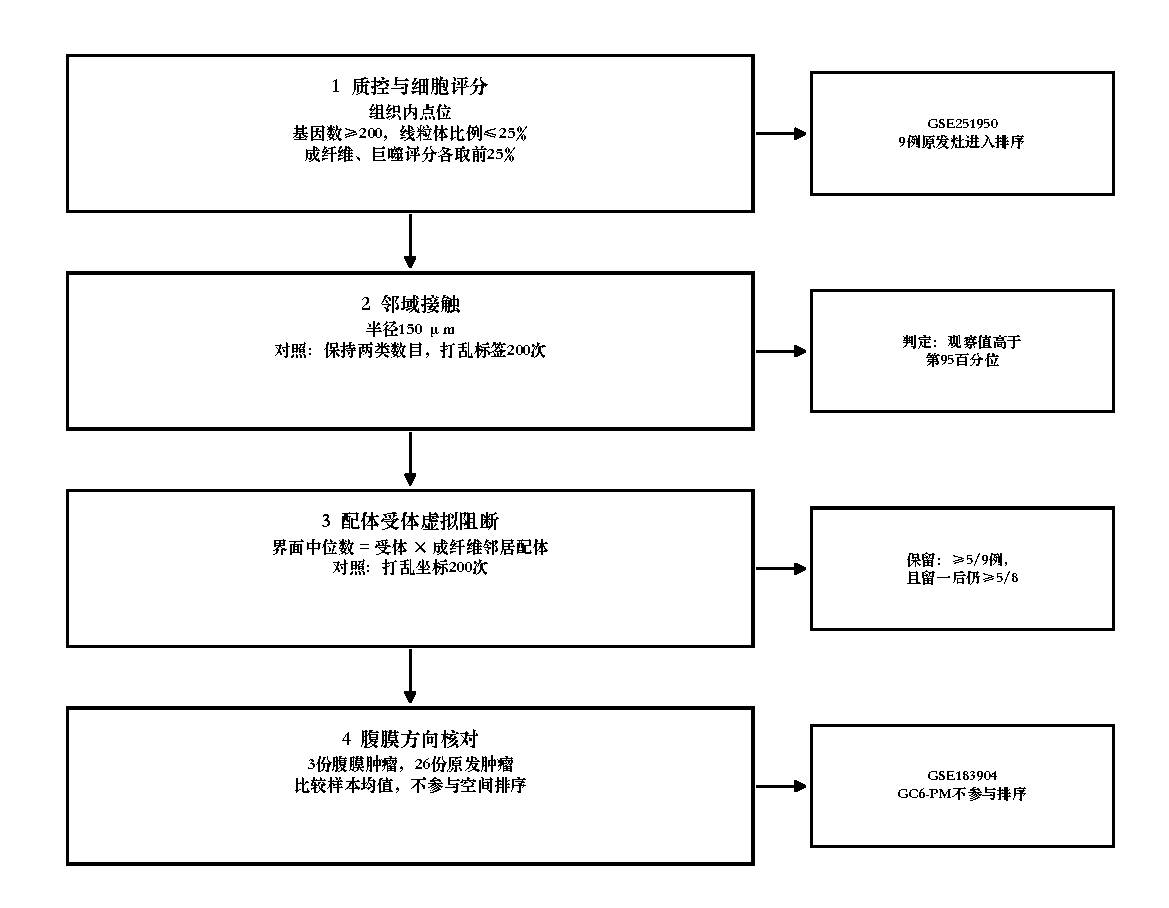
\includegraphics[width=0.92\textwidth]{fig_flow.pdf}
  \caption{四步协议把接触检验、界面信号和腹膜方向分开。右侧为每步的数据或判定，左侧为操作。}
  \label{fig:flow}
\end{figure}

左侧四格按顺序完成质控、150\,$\mu$m接触、界面中位数和腹膜样本均值（图~\ref{fig:flow}）。接触的对照是保持两类数目的标签打乱，界面信号的对照是坐标打乱，两侧都是200次。保留线写在第三步右侧：至少5/9例，且留一后仍至少5/8。第四步的3份腹膜肿瘤和26份原发肿瘤只比较均值，GC6-PM不进入9例排序。半径、分位和这对保留线在出结果之前已经写死，后面的表按这套线报告，不另换阈值。

邻域用点位的显微坐标，半径150\,$\mu$m，由Visium点直径55\,$\mu$m除以全分辨率图像中的点直径像素数换算。配体受体来自CellChat人类库里配体和受体都是单个基因符号的组合，两基因需在全部切片中出现，共1000对。另有5对事先列入：CCL2--CCR2、C3--C3AR1、SPP1--CD44、TGFB1--TGFBR1、TGFB1--TGFBR2。名称里含下划线的复合物没有评分。

在这个可加读数里，去掉一条边之后界面中位数下降的量，就是这条边自己的中位数。报告的检验是该中位数是否高于坐标打乱，而不是边与边争夺同一份通量之后的再分配。单细胞矩阵若呈整数计数，则按细胞做每1万的$\log(1+x)$再对细胞取均值；样本之间比较的是这个均值。

另一次计算不替换上面的保留线。每个点位用四个标志基因程序做非负最小二乘，得到成纤维、巨噬、上皮和T细胞比例，四项加总为1。界面权重是成纤维比例乘巨噬比例。切片读数是该权重下的信号加权平均。空分布把配体表达图平移200、300、400或500\,$\mu$m，方向随机，200次，种子20261004；平移后找不到60\,$\mu$m内真实点位的位置记为缺失。主半径仍是150\,$\mu$m，另报100、200、300\,$\mu$m。9例汇总是中位数，区间来自对9例做2000次有放回抽样。只计算事先点名的配体受体，加上TGFB1乘以TGFBR1与TGFBR2的较小值。不重新筛选1000对，也不再做5/9投票。

同一套四个程序用在GSE183904的细胞上。细胞归入均值最大、且该均值大于0并高于其余三类的那一类；否则不归类。一类少于20个细胞的样本，该类均值不进入中位数。腹膜肿瘤3份对原发肿瘤26份只比方向。

乘积是事后指定的。每份样本先取配体所在类的均值、受体所在类的均值，再相乘。统计量是3份腹膜中位数减去原发中位数。在该条乘积有限的样本里，穷举所有把3份标成腹膜的组合。单侧p是统计量大于等于观察值的组合比例。7条一起做Benjamini--Hochberg。sample38相对sample36只列差值。这个乘积不是CellChat的通讯概率，也不是把一条边从网络里删掉之后的下游变化。

\section{腹膜与原发的类均值乘积}
\label{sec:communication}

这一节把主比较从原发灶点位换成样本。细胞类沿用上一轮的四个程序。乘积用的是类均值，不是把细胞放进CellChat再按细胞数算显著性。7条是看过类均值之后才点名的，所以下面的q不能当成事先锁定的发现。

\begin{figure}[htbp]
  \centering
  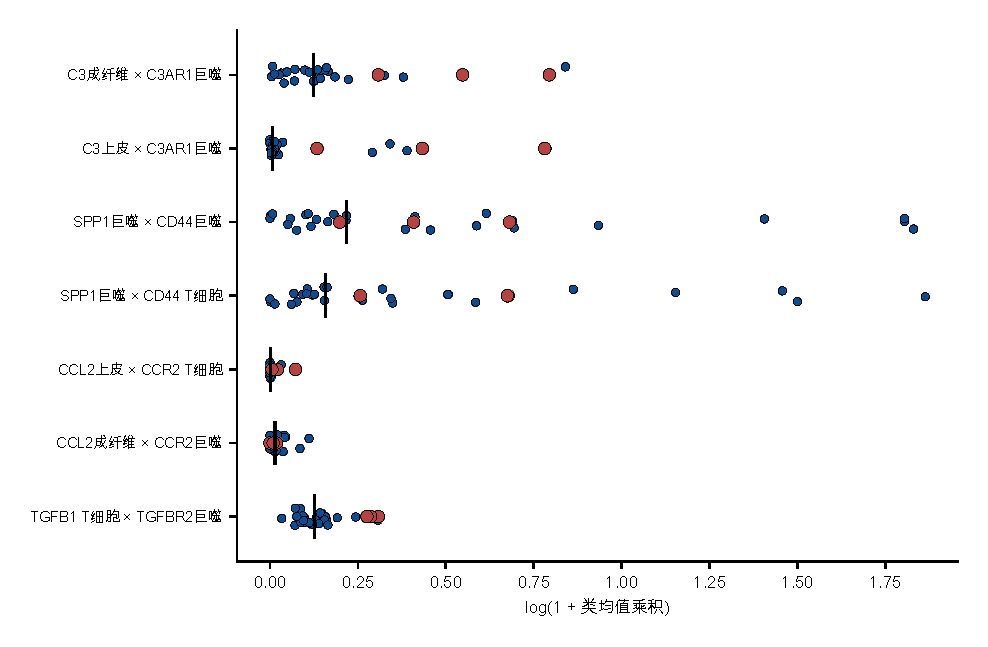
\includegraphics[width=\textwidth]{fig_communication.pdf}
  \caption{每份样本一个乘积。蓝点是原发肿瘤，红点是腹膜肿瘤，黑线是原发中位数。横轴是$\log(1+\text{乘积})$。}
  \label{fig:communication}
\end{figure}

C3上皮乘C3AR1巨噬的腹膜中位数是0.542，原发中位数是0.007，3/3高于原发中位数，置换p为0.004，q为0.027（图~\ref{fig:communication}，表~\ref{tab:communication}）。26份里没有一份原发样本超过这个腹膜中位数，但有3份原发超过腹膜里最低的那一份，两组的范围仍有重叠。C3成纤维乘C3AR1巨噬是0.730对0.132，p为0.015，q为0.027；有1份原发样本高于腹膜中位数。两条都用到巨噬C3AR1，不是两个独立发现。

SPP1巨噬乘CD44巨噬是0.505对0.242，只有2/3高于原发中位数，p为0.42，q为0.49。11份原发样本高于腹膜中位数。巨噬SPP1的类均值在腹膜侧较高，但CD44没有一起升高，乘积站不住。SPP1巨噬乘CD44 T细胞是0.964对0.172，3/3，p为0.094，q为0.13，也不过0.05。

CCL2上皮乘CCR2 T细胞是0.021对0.001，3/3，p为0.015，q为0.027。差值只有0.021。CCL2成纤维乘CCR2巨噬是0.009对0.015，方向相反，p为0.80。这条不能写成腹膜里增强的成纤维--巨噬轴。TGFB1 T细胞乘TGFBR2巨噬是0.332对0.136，p为0.014，q为0.027。来源是T细胞，不是成纤维或巨噬。

\begin{table}[htbp]
  \centering
  \caption{样本水平的类均值乘积。p是穷举3份腹膜标签的单侧比例，q是这7条内部的Benjamini--Hochberg。成纤维或上皮缺失的原发样本是sample22，对应组合数3276；其余为3654。}
  \label{tab:communication}
  \footnotesize
  \setlength{\tabcolsep}{3pt}
  \begin{tabular}{lrrrrr}
    \toprule
    乘积 & 腹膜中位数 & 原发中位数 & 高于原发 & p & q \\
    \midrule
    C3成纤维 $\times$ C3AR1巨噬 & 0.730 & 0.132 & 3/3 & 0.015 & 0.027 \\
    C3上皮 $\times$ C3AR1巨噬 & 0.542 & 0.007 & 3/3 & 0.004 & 0.027 \\
    SPP1巨噬 $\times$ CD44巨噬 & 0.505 & 0.242 & 2/3 & 0.420 & 0.490 \\
    SPP1巨噬 $\times$ CD44 T细胞 & 0.964 & 0.172 & 3/3 & 0.094 & 0.131 \\
    CCL2上皮 $\times$ CCR2 T细胞 & 0.021 & 0.001 & 3/3 & 0.015 & 0.027 \\
    CCL2成纤维 $\times$ CCR2巨噬 & 0.009 & 0.015 & 1/3 & 0.797 & 0.797 \\
    TGFB1 T细胞 $\times$ TGFBR2巨噬 & 0.332 & 0.136 & 3/3 & 0.014 & 0.027 \\
    \bottomrule
  \end{tabular}
\end{table}

同一患者的sample38减sample36，C3上皮乘C3AR1巨噬的差是1.177，C3成纤维乘C3AR1巨噬是1.200。这是1对，不另算p。没有把乘积设成0再去预测STAT3。类均值乘积也不是共培养里的阻断。

巨噬STAT3和SOCS3是另一次样本置换，没有并进上面7条的q。STAT3的腹膜中位数是0.641，原发是0.481，3/3，p为0.010；有1份原发高于腹膜中位数。SOCS3是0.695对0.852，方向相反。两者的均值是0.668对0.623，p为0.47。上皮STAT3也是3/3、p为0.015，所以这不是巨噬独有的升高。这是转录本均值，不是磷酸化，也不是把C3--C3AR1删掉之后的下游变化。

\section{另外三套公开样本}
\label{sec:publicpm}

这三套不和GSE183904混在同一次检验里。7条乘积在下载之前已经写定。GSE308231是3份原发灶对3份腹膜转移实体样本，平台不是10x，记录没有写成同一患者。组合只有20种，单侧p最小是0.05。

\begin{figure}[htbp]
  \centering
  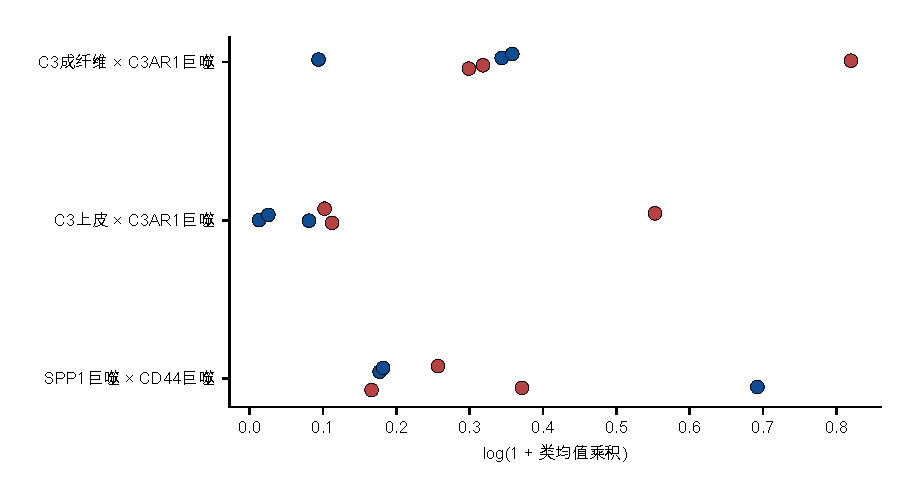
\includegraphics[width=0.92\textwidth]{fig_public_pm.pdf}
  \caption{GSE308231的6份实体样本。蓝点是原发灶，红点是腹膜转移。}
  \label{fig:publicpm}
\end{figure}

7条乘积的q都高于0.35（图~\ref{fig:publicpm}，表~\ref{tab:publicpm}）。C3成纤维乘C3AR1巨噬的腹膜中位数是0.375，原发是0.410，方向相反，p为0.70。C3上皮乘C3AR1巨噬是0.119对0.026，3份腹膜都高于3份原发，p为0.10。换成别的3份标签，中位数差值仍可以达到同样大小，所以p不是0.05。SPP1巨噬乘CD44巨噬是0.293对0.200，p为0.50。

成纤维C3的三份腹膜值是0.949、1.015和1.642，三份原发是0.146、0.664和0.739。上皮C3是0.302、0.314和0.954，对0.019、0.040和0.152。配体在腹膜侧更高。巨噬C3AR1的腹膜中位数是0.395，原发是0.648，没有一起升高。巨噬STAT3是0.697对0.864，SOCS3是0.464对1.195，三份腹膜的SOCS3都低于三份原发。

\begin{table}[htbp]
  \centering
  \caption{GSE308231，3份对3份，穷举20种标签。q是这7条内部的Benjamini--Hochberg。}
  \label{tab:publicpm}
  \footnotesize
  \setlength{\tabcolsep}{4pt}
  \begin{tabular}{lrrrr}
    \toprule
    乘积 & 腹膜中位数 & 原发中位数 & p & q \\
    \midrule
    C3成纤维 $\times$ C3AR1巨噬 & 0.375 & 0.410 & 0.70 & 0.70 \\
    C3上皮 $\times$ C3AR1巨噬 & 0.119 & 0.026 & 0.10 & 0.35 \\
    SPP1巨噬 $\times$ CD44巨噬 & 0.293 & 0.200 & 0.50 & 0.58 \\
    SPP1巨噬 $\times$ CD44 T细胞 & 0.298 & 0.200 & 0.30 & 0.42 \\
    CCL2上皮 $\times$ CCR2 T细胞 & 0.006 & 0.001 & 0.10 & 0.35 \\
    CCL2成纤维 $\times$ CCR2巨噬 & 0.036 & 0.016 & 0.20 & 0.35 \\
    TGFB1 T细胞 $\times$ TGFBR2巨噬 & 0.664 & 0.492 & 0.20 & 0.35 \\
    \bottomrule
  \end{tabular}
\end{table}

GSE163558里标成腹膜转移的只有P1一份，对照是同系列3份原发灶，不算p。P1的C3上皮乘C3AR1巨噬是0.294，原发中位数是0.042；C3成纤维乘C3AR1巨噬是0.309对0.207。P1的巨噬STAT3是0.590，是这4份里最低的一份。

GSE228598是28份腹腔细胞，来自腹水或冲洗液，系列里没有原发灶，也不逐份标明是不是腹膜种植。28份里有15份成纤维细胞少于20个，成纤维均值缺失。有数的13份里，成纤维C3中位数是2.426。全部28份的上皮C3中位数是0.924，巨噬C3AR1是0.829，巨噬STAT3是0.573，SOCS3是0.190。这是腹腔液体，不并入实体瘤的乘积检验。

\section{原发灶空间界面}
\label{sec:results}

9例原发灶上，没有配体受体满足保留规则。接触比例在全部10张切片上都低于标签打乱的第95百分位。

\begin{figure}[htbp]
  \centering
  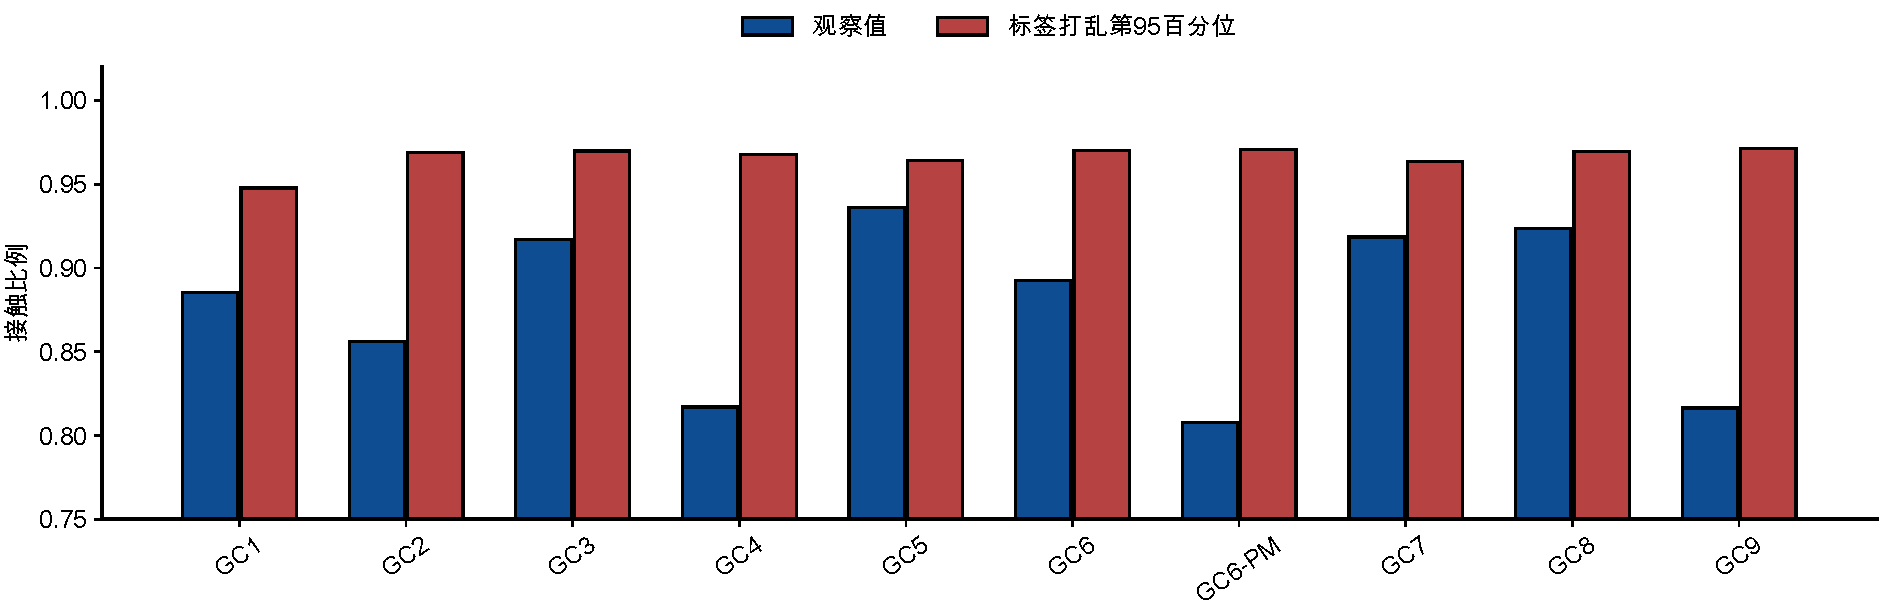
\includegraphics[width=0.96\textwidth]{fig_contact.pdf}
  \caption{10张切片的成纤维--巨噬接触比例都低于标签打乱第95百分位。纵轴从0.75起，以便看清0.81--0.97这一段。}
  \label{fig:contact}
\end{figure}

蓝柱是观察接触比例，红柱是同一张切片上标签打乱200次的第95百分位（图~\ref{fig:contact}）。GC5最高，为0.936，对应空分布0.964；GC6-PM最低，为0.808，对应空分布0.971。9例原发灶的观察值落在0.817--0.936，空分布落在0.948--0.971，没有一例观察值更高。GC4和GC9同为0.817，是原发灶里最低的两例，仍比各自空分布低约0.15。前25\%标签加上150\,$\mu$m半径之后，随机点位本来就很容易碰到成纤维高分区，接触比例因此挤在0.8以上，空分布更靠近0.97。

\begin{table}[htbp]
  \centering
  \caption{事先指定的5对与达到5/9例的3对均未保留。中位数为9例原发灶界面信号的中位数；置换$p$为各切片置换$p$的中位数。}
  \label{tab:main}
  \begin{tabular}{lrrrrl}
    \toprule
    配体受体 & 检出切片 & 过线切片 & 中位数 & 置换$p$中位数 & 留一 \\
    \midrule
    CCL2--CCR2 & 3 & 0 & 0 & 1.000 & 未稳定 \\
    C3--C3AR1 & 9 & 1 & 0 & 1.000 & 未稳定 \\
    SPP1--CD44 & 8 & 1 & 0 & 1.000 & 未稳定 \\
    TGFB1--TGFBR1 & 9 & 2 & 0 & 1.000 & 未稳定 \\
    TGFB1--TGFBR2 & 9 & 3 & 0 & 1.000 & 未稳定 \\
    APP--CD74 & 9 & 5 & 3.37 & 0.030 & 未稳定 \\
    CD99--CD99 & 9 & 5 & 1.68 & 0.030 & 未稳定 \\
    SEMA4D--PLXNB2 & 9 & 5 & 0.13 & 0.040 & 未稳定 \\
    \bottomrule
  \end{tabular}
\end{table}

事先指定的5对，9例界面信号的中位数都是0（表~\ref{tab:main}）。TGFB1--TGFBR2在GC3、GC4、GC5三张切片上高于空分布，是这5对里过线切片最多的一对，仍少于5例。CCL2--CCR2的过线切片数为0；CCR2在界面上的检出比例多低于0.05，9例里只有3例达到预先写出的5\%检出。APP--CD74、CD99--CD99和SEMA4D--PLXNB2各有5例高于空分布，置换$p$的中位数为0.030、0.030和0.040。这3对去掉若干单张切片后，过线数降到5例以下，留一规则没有通过。1000对里被保留的数目为0。

\begin{figure}[htbp]
  \centering
  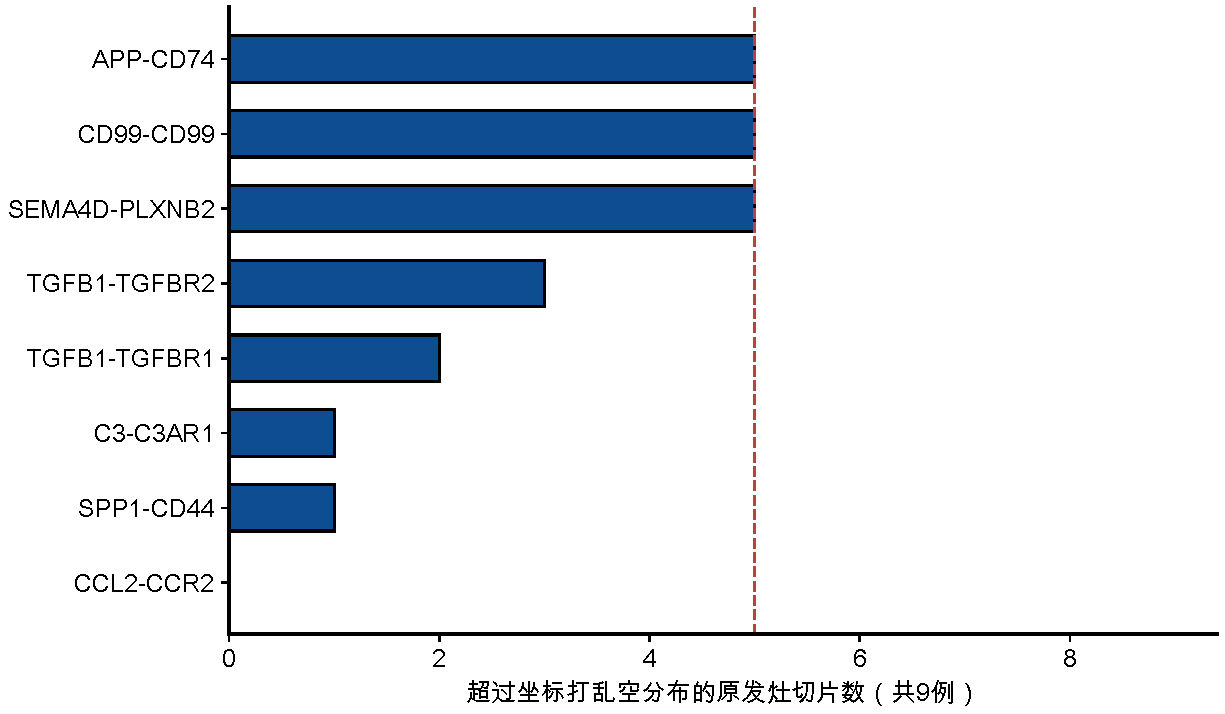
\includegraphics[width=0.78\textwidth]{fig_retention.pdf}
  \caption{虚线是5/9例这一档计数线。三条边碰到虚线，留一之后仍未保留；事先指定的五条边都在虚线左侧。}
  \label{fig:retention}
\end{figure}

横轴是9例原发灶里界面信号高于坐标打乱第95百分位的切片数，虚线标在5（图~\ref{fig:retention}）。APP--CD74、CD99--CD99、SEMA4D--PLXNB2的条形停在5，TGFB1--TGFBR2停在3，C3--C3AR1和SPP1--CD44停在1，CCL2--CCR2为0。停在虚线上只说明过线切片数刚好达到5，表~\ref{tab:main}里这3对的留一列仍是未稳定。胶原和纤连蛋白相关边的界面信号绝对值可以高于1，坐标打乱后的第95百分位同样高，因此没有进入这张计数图的右侧。

\begin{table}[htbp]
  \centering
  \caption{腹膜肿瘤3份与原发肿瘤26份的样本均值。$\log_2$倍数比较两组中位数；配对列是sample38相对sample36。}
  \label{tab:pm}
  \small
  \setlength{\tabcolsep}{4.5pt}
  \begin{tabular}{lrrrrr}
    \toprule
    基因 & 腹膜中位数 & 原发中位数 & $\log_2$倍数 & 高于原发中位数 & 配对$\log_2$ \\
    \midrule
    C3 & 0.876 & 0.045 & 4.24 & 3/3 & 6.41 \\
    SPP1 & 0.129 & 0.041 & 1.62 & 3/3 & 5.17 \\
    CCL2 & 0.183 & 0.136 & 0.43 & 3/3 & 5.20 \\
    CCR2 & 0.019 & 0.012 & 0.56 & 3/3 & 0.87 \\
    TGFBR2 & 0.490 & 0.270 & 0.86 & 3/3 & 0.65 \\
    TGFBR1 & 0.079 & 0.058 & 0.45 & 2/3 & 0.65 \\
    TGFB1 & 0.397 & 0.401 & $-0.01$ & 1/3 & $-0.04$ \\
    CD44 & 0.745 & 0.865 & $-0.21$ & 1/3 & $-0.19$ \\
    \bottomrule
  \end{tabular}
\end{table}

3份腹膜肿瘤的C3样本均值中位数为0.876，26份原发肿瘤为0.045，$\log_2$倍数4.24，3份都高于原发中位数（表~\ref{tab:pm}，图~\ref{fig:pm}）。SPP1为1.62倍的$\log_2$差，CCL2为0.43。配对的sample38相对sample36，C3、SPP1、CCL2的$\log_2$倍数为6.41、5.17和5.20；CCL2的配对倍数大，是因为sample36的均值只有0.003。TGFB1两组中位数为0.397和0.401。CD44腹膜中位数0.745，低于原发的0.865。原发肿瘤里已有C3达到0.56和0.75的样本，3份腹膜肿瘤没有和26份原发肿瘤完全分开。

\begin{figure}[htbp]
  \centering
  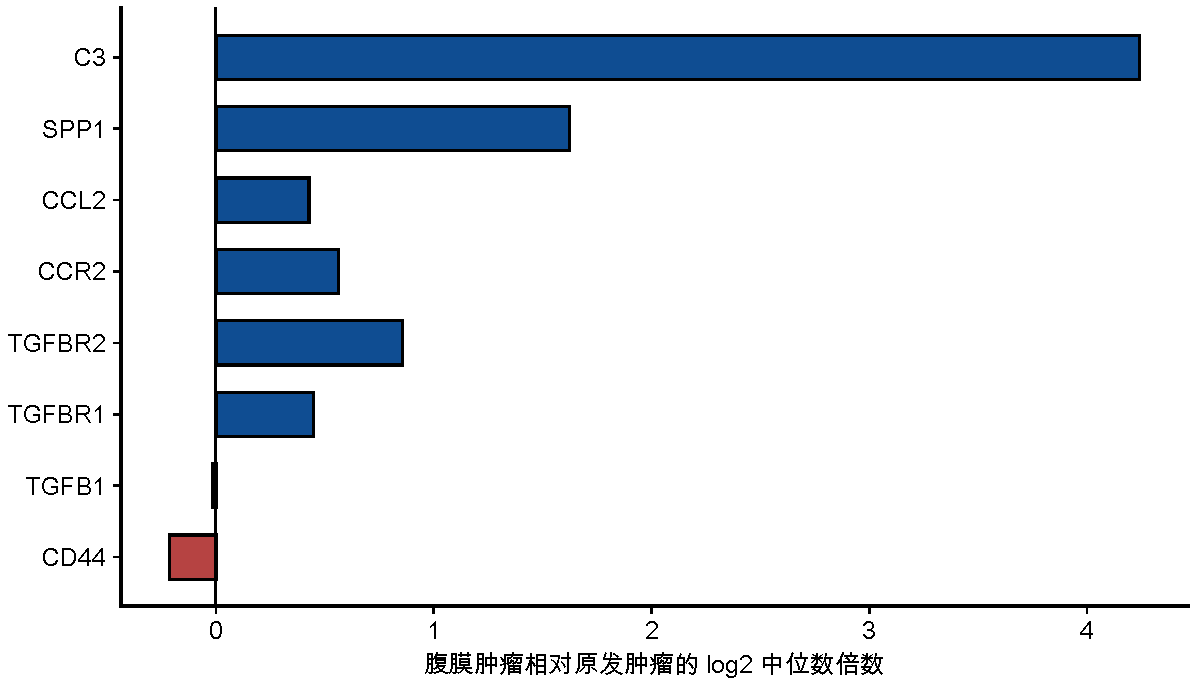
\includegraphics[width=0.72\textwidth]{fig_peritoneal.pdf}
  \caption{C3的腹膜对原发$\log_2$中位数倍数最高。TGFB1接近0，CD44在腹膜侧更低。红柱为负值。}
  \label{fig:pm}
\end{figure}

\section{换一种界面读数}
\label{sec:interface}

第一套规则没有改。这一节是另一次计算：界面不再用前25\%高分区的二值标签，空分布也不再把坐标打乱成互不相关的点。细胞比例用四个标志基因程序的非负最小二乘，不是cell2location。Visium中心距约100\,$\mu$m，50\,$\mu$m和20--50\,$\mu$m的细胞邻接没有算。没有多重免疫荧光、共培养或类器官。

成纤维程序是DCN、LUM、COL1A1、FAP，巨噬程序是CD68、CSF1R、C1QA、C1QB，另有上皮和T细胞程序，用来把比例分开。被检验的配体和受体不进入这四个程序。界面权重是成纤维比例乘巨噬比例。点位信号仍是本点受体乘以150\,$\mu$m邻域的配体均值，切片读数改成权重下的加权平均。空分布把配体图平移200--500\,$\mu$m，200次，种子20261004。9例的汇总是中位数和有放回抽样2000次的区间，不是至少5/9例的投票。GC6-PM不进入这9例。

\begin{figure}[htbp]
  \centering
  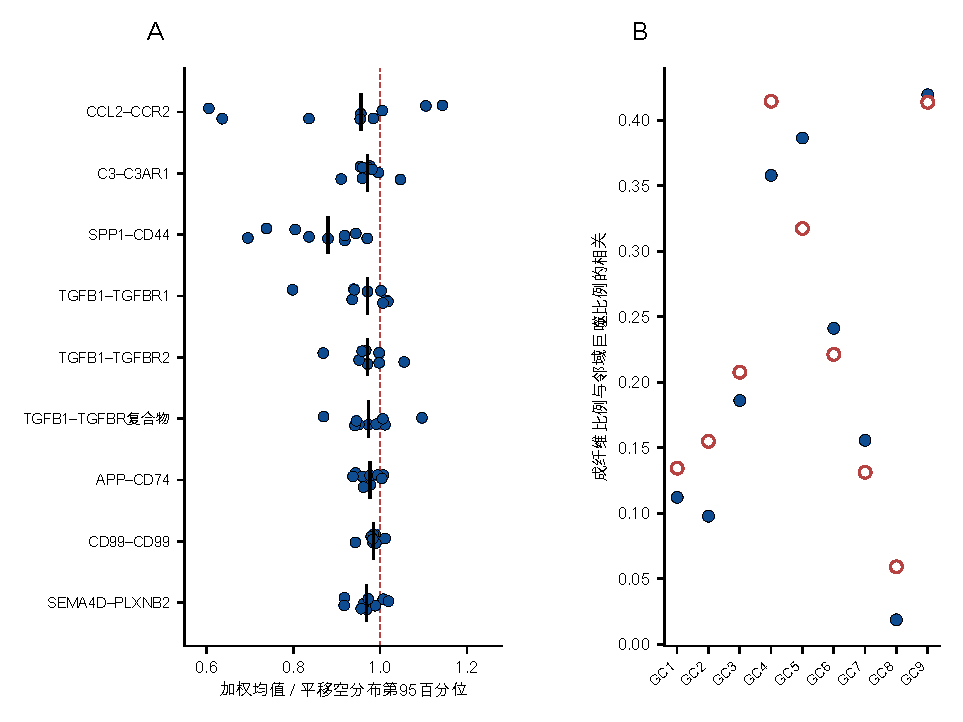
\includegraphics[width=\textwidth]{fig_interface.pdf}
  \caption{平移空分布下的界面读数。A：每个点是一张原发灶切片，横轴是加权均值除以该切片空分布第95百分位，黑线是9例中位数，红虚线是1。B：蓝点是成纤维比例与150\,$\mu$m邻域巨噬比例的相关，红圈是同一张切片上把巨噬比例平移后的第95百分位。}
  \label{fig:interface}
\end{figure}

加权平均把旧分析里被中位数压成0的读数抬了起来，但没有抬到平移空分布之上（图~\ref{fig:interface}，表~\ref{tab:interface}）。C3--C3AR1的9例中位数是0.223，最小到最大是0.092--0.833；超额中位数是$-0.005$，抽样区间$-0.022$到$-0.002$，9例里8例低于自己的空分布。SPP1--CD44的超额在9/9例都为负，中位数$-0.018$，区间$-0.035$到$-0.003$。CCL2--CCR2的加权中位数只有0.012，97\%的界面权重落在信号为0的点位上，超额中位数$-0.001$。CD99--CD99的绝对读数有1.780，超额仍是$-0.021$，区间不跨过0。APP--CD74最高，中位数2.626，超额$-0.068$，区间$-0.136$到0.015，跨过0。SEMA4D--PLXNB2的区间也跨过0。TGFB1与两个受体分开算、再取TGFBR1和TGFBR2的较小值，三条读数的超额中位数都是负的。

\begin{table}[htbp]
  \centering
  \caption{9例原发灶、150\,$\mu$m、比例权重。超额是观察值减去平移空分布第95百分位。括号里是9例中位数经2000次有放回抽样的2.5\%和97.5\%分位。}
  \label{tab:interface}
  \footnotesize
  \setlength{\tabcolsep}{3pt}
  \begin{tabular}{lrrrr}
    \toprule
    配体受体 & 加权中位数 & 最小--最大 & 超额中位数 & 低于空分布 \\
    \midrule
    CCL2--CCR2 & 0.012 & 0.002--0.053 & $-0.001$ ($-0.002$--0.000) & 6/9 \\
    C3--C3AR1 & 0.223 & 0.092--0.833 & $-0.005$ ($-0.022$--$-0.002$) & 8/9 \\
    SPP1--CD44 & 0.088 & 0.007--0.758 & $-0.018$ ($-0.035$--$-0.003$) & 9/9 \\
    TGFB1--TGFBR1 & 0.100 & 0.026--0.198 & $-0.002$ ($-0.007$--0.001) & 5/9 \\
    TGFB1--TGFBR2 & 0.133 & 0.082--0.305 & $-0.006$ ($-0.012$--$-0.0002$) & 8/9 \\
    TGFB1--TGFBR复合物 & 0.060 & 0.014--0.078 & $-0.001$ ($-0.002$--0.001) & 6/9 \\
    APP--CD74 & 2.626 & 1.415--3.990 & $-0.068$ ($-0.136$--0.015) & 7/9 \\
    CD99--CD99 & 1.780 & 0.270--7.242 & $-0.021$ ($-0.032$--$-0.006$) & 8/9 \\
    SEMA4D--PLXNB2 & 0.277 & 0.174--0.723 & $-0.015$ ($-0.023$--0.002) & 7/9 \\
    \bottomrule
  \end{tabular}
\end{table}

半径改成100、200、300\,$\mu$m之后，超额中位数仍在0的负侧。唯一的例外是TGFB1--TGFBR1在100\,$\mu$m的超额中位数为$+0.0001$。把界面改回二值、取中位数，75\%分位以上同时富集成纤维和巨噬的点位上，C3--C3AR1、CCL2--CCR2和TGFB1--TGFBR1的9例中位数都是0。中位数会被零压住；加权平均避开了这个零，却仍不超过保留空间结构的空分布。

成纤维比例和邻域巨噬比例的相关，9例中位数是0.19。4/9例高于平移空分布，超额的中位数是$-0.022$。GC4的相关是0.36，空分布第95百分位是0.41，观察值仍低。第一套里GC4的C3--C3AR1中位数高于坐标打乱，在这一套平移空分布下没有成为稳定超额。

STAT3和SOCS3的转录均值，与C3--C3AR1、CCL2--CCR2、SPP1--CD44点位信号的Spearman中位数是0.08、0.02和0.15，没有一张切片超过0.21。这是转录本上的相关，不是磷酸化，也不是把一条边从网络里删掉之后的下游变化。

GC6-PM的C3--C3AR1加权均值是0.922，平移空分布第95百分位是0.925，超额$-0.004$。绝对水平和原发灶不是同一档，仍没有高于这张切片自己的空分布。它的转移部位记录不是腹膜，不并入9例。

单细胞按同一套程序归类。原发灶sample22只有6个成纤维细胞和18个上皮细胞，这两类不进入中位数，所以成纤维和上皮的原发分母是25份，巨噬和T细胞是26份。3份腹膜对原发只报方向（表~\ref{tab:source}）。

C3在原发灶里成纤维中位数最高，为0.374。3份腹膜肿瘤的成纤维中位数是2.032，3/3高于原发中位数；上皮是0.958对0.031，也是3/3。sample19和sample38里最高的一类是成纤维，sample20是上皮。SPP1在原发灶和腹膜里都以巨噬最高，腹膜巨噬中位数0.729，原发0.211，2/3高于原发。成纤维两边都低，0.068对0.053。sample19这一份里最高的一类是上皮。

CCL2在原发灶成纤维的中位数是1.084。3份腹膜成纤维中位数是0.422，0/3高于原发。前面样本均值里CCL2的腹膜方向，不是成纤维升高。腹膜里CCL2最高的类也不固定：sample19和sample38是上皮，sample20是巨噬。上皮中位数0.250对0.054，3/3高于原发，绝对值仍低于原发成纤维。TGFB1在3份腹膜里最高的类都是T细胞，中位数0.802对0.565，3/3；成纤维和巨噬都是1/3。

受体这边，C3AR1落在巨噬，腹膜中位数0.566，原发0.342，3/3。CCR2在腹膜T细胞的中位数是0.085，高于巨噬的0.045。CD44在巨噬和T细胞上都高，腹膜巨噬中位数1.076，低于原发巨噬1.251。

\begin{table}[htbp]
  \centering
  \caption{GSE183904按细胞类的样本均值。腹膜肿瘤3份，原发肿瘤成纤维和上皮25份、巨噬和T细胞26份。高于原发中位数的计数只作方向。}
  \label{tab:source}
  \footnotesize
  \setlength{\tabcolsep}{4pt}
  \begin{tabular}{llrrr}
    \toprule
    基因 & 细胞类 & 腹膜中位数 & 原发中位数 & 高于原发 \\
    \midrule
    C3 & 成纤维 & 2.032 & 0.374 & 3/3 \\
    C3 & 巨噬 & 0.834 & 0.085 & 2/3 \\
    C3 & 上皮 & 0.958 & 0.031 & 3/3 \\
    C3 & T细胞 & 0.087 & 0.003 & 3/3 \\
    SPP1 & 成纤维 & 0.068 & 0.053 & 2/3 \\
    SPP1 & 巨噬 & 0.729 & 0.211 & 2/3 \\
    SPP1 & 上皮 & 0.065 & 0.018 & 2/3 \\
    SPP1 & T细胞 & 0.020 & 0.009 & 3/3 \\
    CCL2 & 成纤维 & 0.422 & 1.084 & 0/3 \\
    CCL2 & 巨噬 & 0.217 & 0.290 & 1/3 \\
    CCL2 & 上皮 & 0.250 & 0.054 & 3/3 \\
    CCL2 & T细胞 & 0.021 & 0.008 & 3/3 \\
    TGFB1 & 成纤维 & 0.226 & 0.443 & 1/3 \\
    TGFB1 & 巨噬 & 0.480 & 0.535 & 1/3 \\
    TGFB1 & 上皮 & 0.327 & 0.230 & 2/3 \\
    TGFB1 & T细胞 & 0.802 & 0.565 & 3/3 \\
    \bottomrule
  \end{tabular}
\end{table}

\section{诊断与稳健性}
\label{sec:diagnostics}

界面中位数对稀疏受体几乎没有区分度。9000个原发灶配体受体--切片组合里，界面中位数大于0的占6.1\%。1000对里，9例中位数等于0的占95.3\%。C3在成纤维高分区的检出比例可以到0.50--0.96，C3AR1在界面上多为0.14--0.36，乘积仍有超过一半的界面点位为0，中位数因此落在0。GC4是例外：C3--C3AR1的界面中位数为0.912，空分布第95百分位为0.845，置换$p$为0.005。把9例再取中位数时，这一例被其余8个0盖住。

留一规则比“刚好5例”更紧。APP--CD74的5例过线分布在部分切片上，去掉GC1、GC4、GC6、GC8或GC9中的任意一张，过线数就少于5。CD99--CD99和SEMA4D--PLXNB2同样卡在5例。置换次数为200，第95百分位对应的切片内置换$p$约为0.05；中位数置换$p$为0.030，表示至少一半切片的置换$p$不高于这个量级，另一半可以接近1。因此5/9过线不等于9例一致。

接触比例的空分布集中在0.95--0.97，观察值集中在0.81--0.94。两组都高，差值的方向在10张切片上一致：观察值更低。这个方向说明当前半径和前25\%阈值下，真实标签的接触不多于随机标签。

\section{讨论}
\label{sec:discussion}

腹膜侧能站住的是样本中位数，不是空间邻接，也不是下游功能。C3上皮或成纤维乘巨噬C3AR1，在3份对25份的标签置换里q为0.027。这个q只覆盖事后点名的7条，而且两条C3共用同一个受体。SPP1巨噬乘CD44巨噬的q是0.49，不能和C3写成同一条已经增强的通讯。CCL2若从上皮接到T细胞的CCR2，q也是0.027，但乘积只有0.021；从成纤维接到巨噬CCR2则没有升高。TGFB1的乘积来自T细胞。

这些样本来自已经发表的胃癌单细胞队列。这里的置换只说明在这份公开数据里，3份腹膜肿瘤的C3乘积位于原发样本的高侧。巨噬STAT3转录均值也偏高，SOCS3没有一起升高，不能写成STAT3活性已经上来。GSE308231的3对3没有复现这个乘积：成纤维C3乘巨噬C3AR1的腹膜中位数更低，7条q都高于0.35。它不增加已经通过检验的样本量，也不代替蛋白邻近或受体阻断。

原发灶的保留规则收成0对。APP--CD74等3对达到5/9例，界面中位数也明显高于事先指定的5对，但留一后过线数下降，不能写成在9例上都站得住的边。事先指定的TGFB1--TGFBR2最多3例过线，中位数仍为0，和“至少5例且留一稳定”之间差了留一和切片数两道。

接触比例低于空分布，和界面信号里大量0中位数是同一几何条件的两面。150\,$\mu$m已经盖住Visium相邻点位，前25\%又使成纤维高分区足够密，随机标签的接触比例被推到0.97附近。观察值低于这条线，说明在这个定义下看不到超出随机的邻域富集。胶原、纤连蛋白相关边的绝对信号高，是因为配体和受体在很多点位上都有表达；坐标打乱后信号仍高，所以绝对值和空间超额是两件分开的事。

腹膜样本均值里，C3、SPP1、CCL2在3份腹膜肿瘤上都高于原发中位数，配对患者上也同向。空间检验里，C3--C3AR1和SPP1--CD44只在1/9例原发灶上超过坐标打乱，CCL2--CCR2为0/9。表达方向和界面超额因此没有落在同一批边上。TGFB1的两组中位数几乎相同，空间上TGFB1--TGFBR2也只有3例过线。3份腹膜样本不能把这种方向写成腹膜特异的阻断顺序。

把中位数换成比例加权、把坐标打乱换成配体图平移，绝对读数不再全是0，超额仍然站在空分布下面。这说明第一套的阴性结果不单是中位数被零压住。半径从100改到300\,$\mu$m，方向不变。GC4在旧空分布下的那一个C3--C3AR1过线，没有在平移空分布下变成9例的超额。

单细胞分类把三条腹膜方向拆开了。C3在成纤维和上皮里都高于原发中位数，SPP1主要在巨噬，CCL2的腹膜样本均值并不是成纤维升高。3份对26份仍只是方向。

\section{局限}
\label{sec:limitations}

\begin{itemize}
  \item 空间单位是Visium点位。点直径约55\,$\mu$m，中心距约100\,$\mu$m。150\,$\mu$m邻域不是细胞之间的距离。
  \item 排序用的独立切片是9例原发灶。GC6-PM只有1张，且转移部位没有写成腹膜。
  \item 腹膜肿瘤3份，其中只有1对与原发灶来自同一患者。样本均值方向没有置信区间，也不做显著性声明。
  \item 界面读数是可加乘积的中位数。它不描述配体受体之间的竞争，也不等于药物阻断后的细胞状态。
  \item CellChat库中带下划线的复合物受体没有进入1000对。TGFB受体在库里的复合物名称因此没有替代TGFBR1、TGFBR2这两行单基因。
  \item 接触空分布和界面空分布都接近饱和或零膨胀。换半径、换分位或改用均值，会是另一套规则，本报告不把那种替换后的排序当作当前结果。
  \item 比例加权和平移空分布仍在Visium点位上。它不是单细胞邻域，也不是把一条边从通讯网络中删除后的下游变化。没有蛋白染色和共培养。
  \item 腹膜乘积是看过类均值之后指定的7条。q只在这7条内部计算。3份腹膜肿瘤不能把C3乘积写成已经验证的免疫抑制轴。GSE308231只有3对3，p最小是0.05，而且没有复现这个乘积。
\end{itemize}

\section{结论}
\label{sec:conclusion}

\begin{enumerate}
  \item C3上皮乘C3AR1巨噬、C3成纤维乘C3AR1巨噬，在3份腹膜肿瘤对原发肿瘤的样本置换里q为0.027。两条共用巨噬C3AR1，而且是看过类均值之后才检验的。
  \item SPP1巨噬乘CD44巨噬的q为0.49。腹膜CD44没有随SPP1一起升高。巨噬STAT3转录均值的置换p为0.010，SOCS3没有升高，两者均值的p为0.47。
  \item CCL2成纤维乘CCR2巨噬的腹膜中位数低于原发。CCL2上皮乘CCR2 T细胞的q为0.027，乘积差值是0.021。
  \item 10张切片的成纤维--巨噬接触比例为0.81--0.94，全部低于标签打乱第95百分位0.95--0.97。
  \item 1000对配体受体里，没有一对在9例原发灶上同时满足至少5例超过坐标打乱、且留一后仍至少5/8。
  \item 事先指定的CCL2--CCR2、C3--C3AR1、SPP1--CD44、TGFB1--TGFBR1和TGFB1--TGFBR2，9例界面中位数都是0。比例加权和平移空分布之后，超额中位数仍不超过0。
  \item GSE308231的3份腹膜实体瘤对3份原发灶，7条乘积的q都高于0.35。C3成纤维乘C3AR1巨噬的腹膜中位数低于原发。上皮C3和成纤维C3更高，巨噬C3AR1和SOCS3没有一起升高。
\end{enumerate}


\begin{thebibliography}{9}
\bibitem{gut2025}
Spatial dissection of tumour microenvironments in gastric cancers reveals the immunosuppressive crosstalk between CCL2$^{+}$ fibroblasts and STAT3-activated macrophages.
\textit{Gut}. 2025;74:714.
doi:10.1136/gutjnl-2024-332901.
\bibitem{kumar2022}
Kumar V, Ramnarayanan K, Sundar R, et al.
Single-cell atlas of lineage states, tumor microenvironment, and subtype-specific expression programs in gastric cancer.
\textit{Cancer Discovery}. 2022.
PMID:34642171.
\end{thebibliography}

\end{document}
